\subsection{Full system}

\begin{figure}[htbp]
   \centerline{
   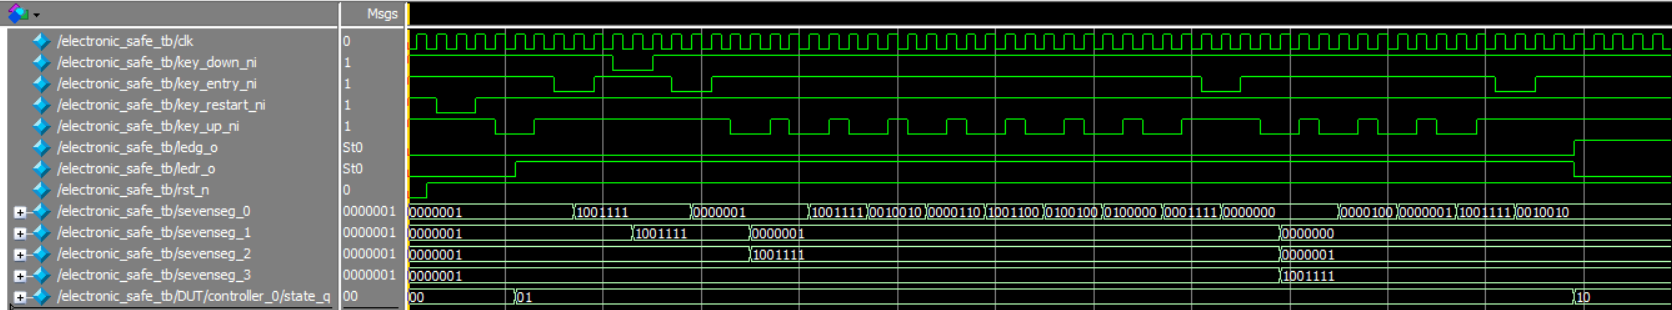
\includegraphics[width=\paperwidth]{full_sys_sim.png}}
   \caption{Full system simulation in ModelSim.}
   \label{fig:full_sys_sim}
\end{figure}

Fig.~\ref{fig:full_sys_sim} is the full system simulation result in ModelSim. The system was started by released reset and pressed restart key, which was indicated by the controller's state transitived from 00 (Idle) to 01 (Entering) at the bottom line. The red led was turned on after the system started. By entering up, down, and entry keys, the user input digits were stored in the shift register. The seven segment decoders read digits from the shift register and displayed them. After user input every digits, the system went into 10 (Entered) state. In the Entered state, the user input digits were compared with the pin stored in the device. The user input digits matched with the pin, and the green led turned on and red led turned off. The system can be restarted by pressing the restart key.

\begin{figure}[htbp]
   \centerline{
   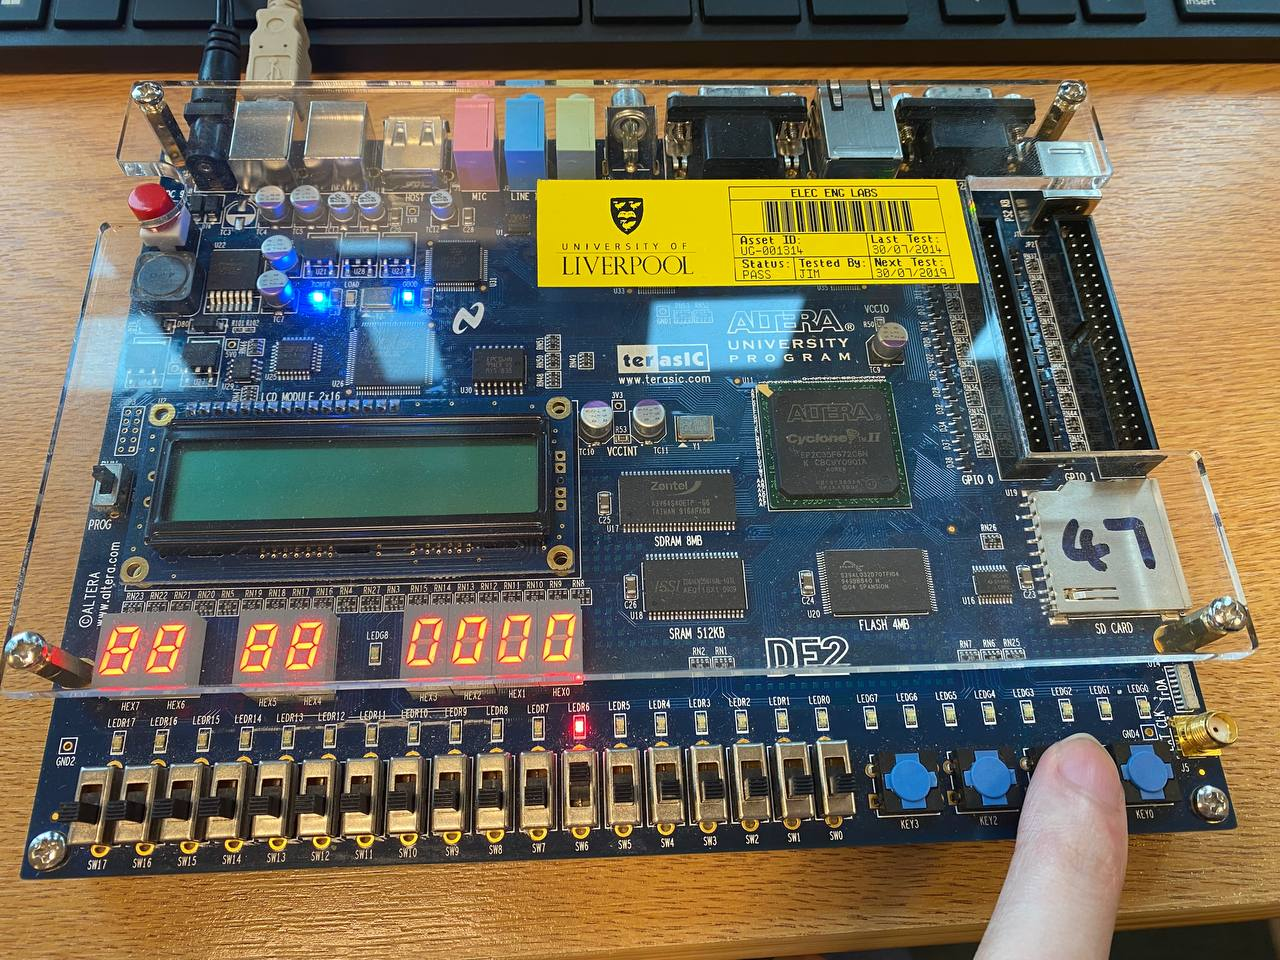
\includegraphics[width=\paperwidth]{entering.jpeg}}
   \caption{Reset switch was released and restart key was pressed.}
   \label{fig:entering}
\end{figure}

\begin{figure}[htbp]
   \centerline{
   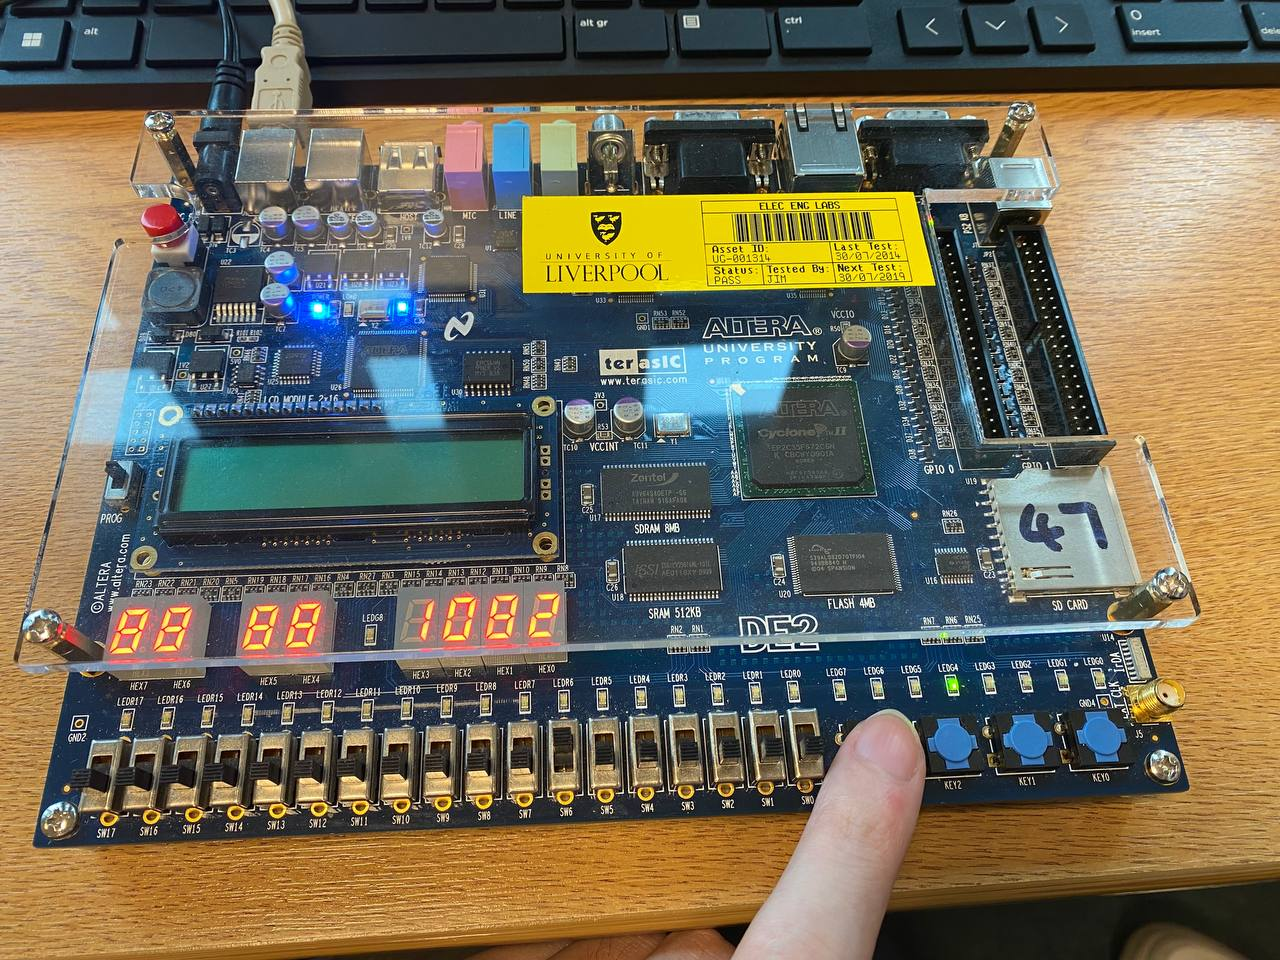
\includegraphics[width=\paperwidth]{entered.jpeg}}
   \caption{Pin was entered correctly.}
   \label{fig:entered}
\end{figure}

\begin{figure}[htbp]
   \centerline{
   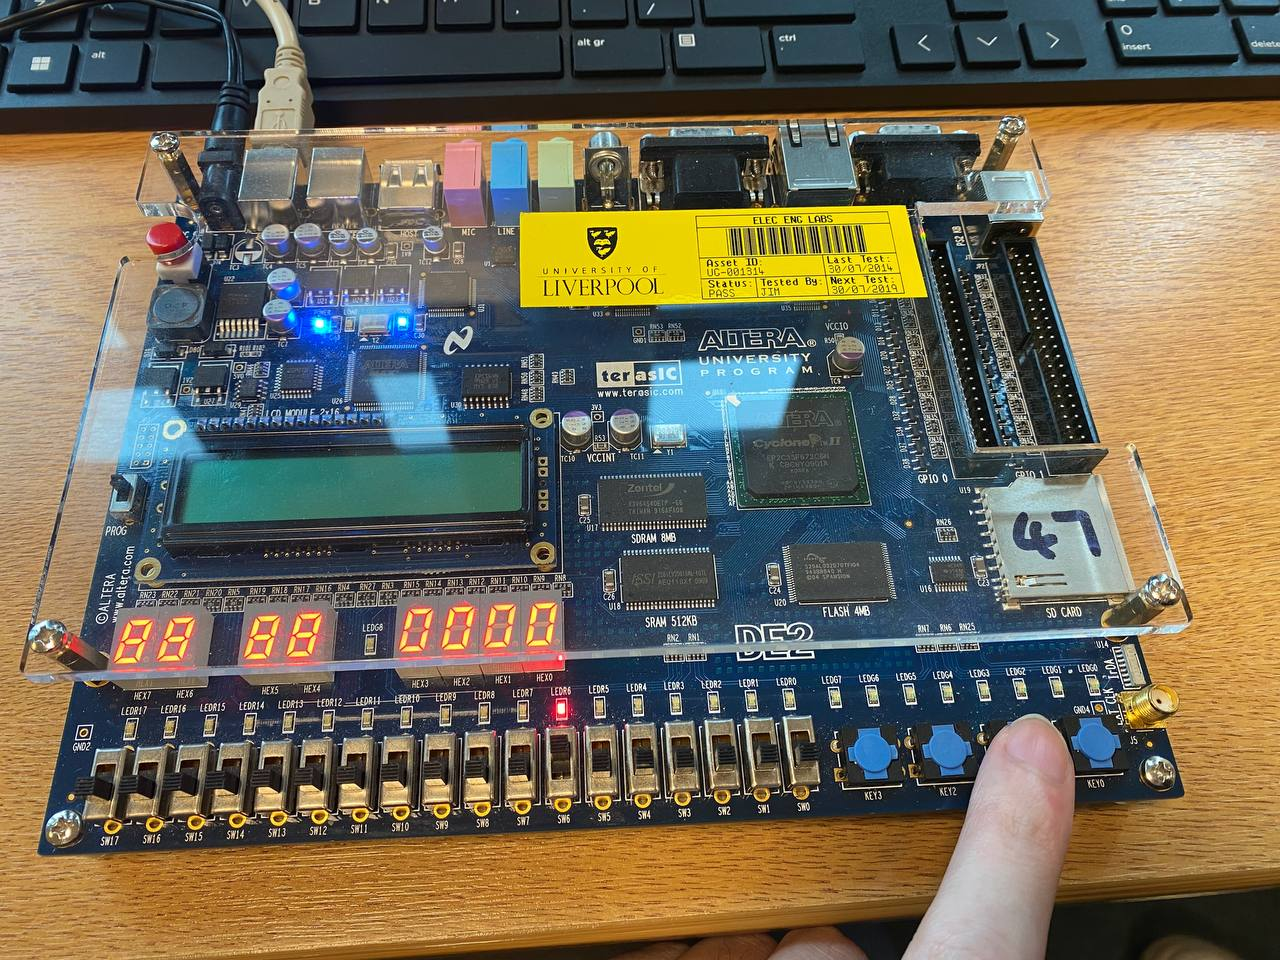
\includegraphics[width=\paperwidth]{restarted.jpeg}}
   \caption{Restart key was pressed and the system was locked and went back to the entering state.}
   \label{fig:restarted}
\end{figure}
